\section{Reliable 1Pipe}
\label{sec:reliable}

Now, we design reliable \sys{} that handles packet loss and failure.
When a receiver delivers a message with timestamp $T$, it must make sure that all messages below $T$ are delivered.
So, if a receiver is unaware of packet loss, it cannot reliably deliver messages according to the barrier timestamp.
In-network packet loss detection still does not solve the problem, because \emph{host failure and packet loss may happen together}.
Consider an example where host $A$ sends to $B$, and then sends to $C$ via a different network path. The packet $A \rightarrow B$ is lost on the way. Then, $A$ crashes. The packet $A \rightarrow C$ is delivered, while $A \rightarrow B$ cannot be recovered. Failure to deliver $A \rightarrow B$ and delivery of $A \rightarrow C$ violates reliable ordering property.
Although the probability of simultaneous packet loss and host failure is very low, a reliable service still needs to take this into account.


\begin{figure}[t]
\centering
	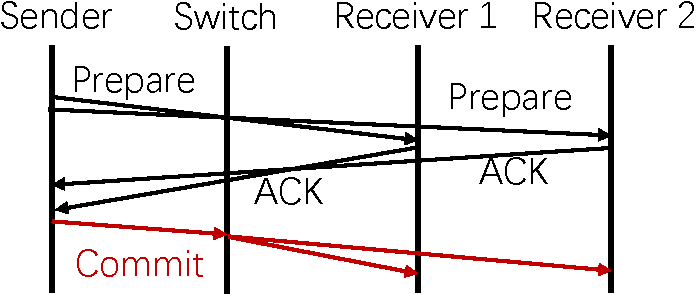
\includegraphics[width=.3\textwidth]{images/2PC.pdf}
	\caption{Two Phase Commit in reliable \sys{}.}
	\label{fig:2PC}
\end{figure}

The key idea of reliable \sys{} is a \emph{Two Phase Commit (2PC)} approach, as Figure~\ref{fig:2PC} shows:

\begin{ecompact}
\item \textbf{Prepare phase}: Sender puts messages into send buffer, and transmits them with timestamps. Network switches do NOT need to aggregate timestamp barriers. Receivers store the messages in receive buffer, and respond with ACKs. Senders wait for end-to-end ACKs, and retransmit messages if packets are lost in-flight. Packet loss detection is end-to-end (as in TCP).
\item \textbf{Commit phase}: When a sender collects all ACKs below or equal to $T$, it sends a \emph{commit message} that carries timestamp $T$ and \emph{commit barrier} $T$. Each network switch aggregates minimum commit barriers on input links, and produce commit barriers to propagate to output links. This timestamp aggregation procedure is exactly the same as Sec.~\ref{sec:loss-free}. A receiver delivers messages below or equal to $T$ in receive buffer when it receives a commit barrier $T$.
\end{ecompact}



\parab{Failures of processes, hosts, switches, and links.}
Like in Sec.~\ref{sec:beacon}, crash failure of a component is detected by its neighbors not hearing any message after a timeout.
However, a failed component cannot be simply removed as in Sec.~\ref{sec:beacon}, because otherwise, the in-flight messages sent by the failed component cannot be consistently delivered or discarded.

To achieve restricted failure atomicity in Sec.\ref{subsec:abstration}, we use the network controller in data centers as a perfect failure detector~\cite{chandra1996unreliable}, which collects failure timestamps of processes and broadcasts them to all correct processes.
The controller itself is replicated using Paxos~\cite{lamport1998part} or Raft~\cite{raft}, so, it is highly available, and only one controller is active at any time.

The procedure to handle failure is as follows: (see Appendix for correctness analysis)

\begin{ecompact}
\item \textbf{Detect}: The neighbors of failed components notifies controller along with its last commit timestamp $T$.
\item \textbf{Determine}: Controller determines \emph{failed processes} and their \emph{failure timestamps} from failed components based on routing graph (Figure~\ref{fig:dcn}). \emph{A process that disconnects from controller in routing graph is regarded as failed}.
%For example, if a host or the only network link from a host fails, all processes on it are disconnected from the data center network, so they are considered to fail simultaneously.
%If a Top-of-Rack (ToR) switch fails, and hosts in the rack are only connected to one switch, then all processes in the rack are considered to fail.
Failure timestamp of a process $P$ is a commit timestamp sent by $P$ but not propagated to any receiver, which is computed as the maximum last commit timestamp reported by all neighbors of $P$ (formally, a cut in routing graph that separates $P$ and all receivers).
If severe network partition occurs and controller cannot access such a cut, controller may either wait for recovery or sacrifice atomicity between isolated partitions.
%If a Leaf, Spine, or Core switch fails, and the connectivity among hosts is not interrupted, no process is considered to fail.
%If network partition occurs, only one partition may connect to controller, and controller will announce failure of all processes in other network partitions.
\item \textbf{Broadcast}: Controller broadcasts the failed processes $P$ and its failure timestamp $T$ to all correct processes.
\item \textbf{Discard}: Each correct process discards messages sent from $P$ with timestamp higher than $T$ in receive buffer.
\item \textbf{Recall}: Each correct process discards messages sent to $P$ in send buffer, which are waiting for ACK from $P$. If a discarded message is in a batch, according to failure atomicity, the batch needs to be aborted, \emph{i.e.}, messages to other receivers \emph{in the same batch} need to be recalled. The sender sends a \emph{recall} message to such receivers, then each of the receivers discards the messages in receive buffer, and responds ACK to the sender. The sender completes Recall after collecting the ACKs.
\item \textbf{Callback}: Each correct process executes the process failure callback registered in Table~\ref{tab:abstraction}, which enables applications to customize failure handling. Then, it responds controller with a completion message.
\item \textbf{Resume}: Controller collects completions from all correct processes.
After all failed processes have been handled by all correct processes, controller notifies network components to remove input link from the failed component, thereby resuming barrier propagation.
%Before this step, commit barrier $T$ from $P$ is never delivered.
\end{ecompact}

\parab{Liveness Mechanism.} If a network failure affects connectivity between $S$ and $R$, the Commit phase in 2PC and the Recall step in failure handling may stall. %$S$ repeatedly retransmits a message but cannot receive ACK from $R$.
In this case, $S$ asks controller to forward the message to $R$, and waits for ACK from controller. If controller also cannot deliver the message, $R$ will be announced as failed, and the undeliverable recall message is recorded. If controller receives ACK of a recall message but cannot forward it to $S$, $S$ will be announced as failed. In summary, if a process does not respond controller within timeout, it is considered as failed.

\parab{Receiver Recovery.} If a process recovers from failure (\emph{e.g.}, the network link or switch recovers), it needs to consistently deliver or discard messages in receive buffer. The controller notifies process of its own failure. Then, the process contacts controller to get host failure notifications since its failure and undeliverable recall messages that are stored at controller. A message with timestamp $T$ in receive buffer is delivered if and only if it is not recalled and the sender is correct at $T$. After delivering buffered messages, because \sys{} assumes a fail-stop model to avoid repeated failure of a process, the recovered process needs to join \sys{} as a new process.

%The 2PC procedure ensures that if a message $M$ from $S$ to $R$ with timestamp $T$ is delivered, then all messages from $S$ and below $T$ have been buffered in their corresponding receivers. If the receiver $R$ is correct when it receives commit barrier $T$, $M$ should be delivered.
%In addition, timestamp aggregation ensures that if a message to $R$ with $T$ is committed, all messages to $R$ below $T$ are also committed.

%The Discard step of failure handling ensures that a message $M: S \rightarrow R$ with timestamp $T$ is not delivered if $S$ fails before $T$. The Recall step ensures that if $M: S \rightarrow R$ and $M': S \rightarrow R'$ are in the same batch, $M$ is not delivered if $R'$ fails before $T$.

%Although the failure recovery process requires the controller to broadcast to all correct processes, it is only invoked when failure occurs, so, the overhead is limited.


%Consider crash failure only. No Byzantine failure. Controller is a perfect failure detector: every faulty process is eventually permanently suspected by every non-faulty process. Non-faulty process are never suspected. Controller itself is replicated using traditional Paxos / Raft.

%only guarantees reliable delivery in absence of host failure during packet loss recovery. Because packet loss is rare and host failure is infrequent, combined probability is very low. When host fail, cannot recover lost packets, but other packets may have delivered.